\documentclass[a4paper, 12pt, twoside]{article}
\usepackage[hungarian]{babel}
\usepackage{ae,aecompl}
\usepackage[T1]{fontenc}
\usepackage[utf8]{inputenc}
\usepackage{textcomp}
\usepackage{pgfplots}
\usepackage{anysize}
% left right up down
\marginsize{3.2cm}{2.8cm}{2cm}{2cm}
\usepackage{setspace}
\setstretch{1.2}
\frenchspacing
\pgfplotsset{compat=newest}
%\pagestyle{empty}
\usepgfplotslibrary{ternary}
\usepackage{chemfig}
\usepackage{gensymb}
\usepackage{fancyhdr}
\usepackage{enumerate}
\usepackage{amsmath}
\usepackage{upgreek}
\numberwithin{equation}{section}
\numberwithin{figure}{section}
\numberwithin{table}{section}
\hyphenation{hő-mér-sék-let-füg-gé-sét}

\renewcommand\footrule{\begin{minipage}{1\textwidth}
%\hrule width \hsize height 2pt \kern 1mm \hrule width \hsize   
\hrule width \hsize height 1pt   
\end{minipage}\par}%

\renewcommand\headrule{
\begin{minipage}{1\textwidth}
%\hrule width \hsize \kern 1mm \hrule width \hsize height 2pt 
\hrule width \hsize height 1pt 
\end{minipage}}%

\pagestyle{fancy}
\fancyhf{}
%\fancyhead[LE,RO]{\leftmark}

%\setlength{\footskip}{40pt}

%\pagestyle{fancy}
%\fancyhf{}
%\usepackage{lastpage}
%\rfoot{Page \thepage \hspace{1pt} of \pageref{LastPage}}
%\lhead{\thesection}
%\cfoot{\itshape\textcolor{gray}{Fizikai Kémia gyakorlatok gyógyszerészeknek}}

\setcounter{tocdepth}{1}
%\thispagestyle{empty}
\title{Fizikai Kémia gyakorlatok}
\author{Kovács Barna \\ Kunsági-Máté Sándor \\ Kiss András}
\date{}
 
\begin{document}
%\clearpage\maketitle
%\thispagestyle{empty}
%\newpage 
%\tableofcontents
%\newpage

%\documentclass[a4paper, 12pt, twoside]{article}
\usepackage[hungarian]{babel}
\usepackage{ae,aecompl}
\usepackage[T1]{fontenc}
\usepackage[utf8]{inputenc}
\usepackage{textcomp}
\usepackage{pgfplots}
\usepackage{anysize}
\marginsize{3.2cm}{2.8cm}{3cm}{2cm}
\usepackage{setspace}
\setstretch{1.2}
\frenchspacing
\pgfplotsset{compat=newest}
%\pagestyle{empty}
\usepgfplotslibrary{ternary}
\usepackage{chemfig}
\usepackage{gensymb}
\usepackage{fancyhdr}
\usepackage{enumerate}

\hyphenation{hő-mér-sék-let-füg-gé-sét}

\renewcommand\footrule{\begin{minipage}{1\textwidth}
\hrule width \hsize height 2pt \kern 1mm \hrule width \hsize   
%\hrule width \hsize height 1pt   
\end{minipage}\par}%

\renewcommand\headrule{
\begin{minipage}{1\textwidth}
\hrule width \hsize \kern 1mm \hrule width \hsize height 2pt 
\end{minipage}}%

\pagestyle{fancy}
\fancyhf{}
%\fancyhead[LE,RO]{\leftmark}
\fancyhead[LE,RO]{GYÓGYSZERBOMLÁS -- ,,GYB''}
\fancyhead[LO,RE]{\thesection}
\fancyfoot[LE,RO]{\thepage}
\fancyfoot[RE,LO]{\emph{Fizikai Kémia gyakorlatok gyógyszerész hallgatóknak}}

%\setlength{\footskip}{40pt}

%\pagestyle{fancy}
%\fancyhf{}
%\usepackage{lastpage}
%\rfoot{Page \thepage \hspace{1pt} of \pageref{LastPage}}
%\lhead{\thesection}
%\cfoot{\itshape\textcolor{gray}{Fizikai Kémia gyakorlatok gyógyszerészeknek}}

\begin{document}

\setcounter{section}{7}
\section{Gyógyszerbomlás sebességének hőmérsékletfüggése}
\subsection{Bevezetés}

A gyakorlat során az \emph{Aspirin} (acetilszalicilsav) hidrolízisének kinetikailag elsőrendű reakciójának hőmérsékletfüggését vizsgáljuk.
A sebességi állandója a következőképpen adható meg:

\begin{equation}
\label{eq:divider}
        k
        =
        \frac
                {1}
                {t}
	\ln
	\frac{z}{z-x}
\end{equation}

ahol $t$ az idő, $z$ a reagens (jelen esetben a \emph{Aspirin}) kezdeti koncentrációja, $x$ pedig az elbomlott reagens koncentrációja.

A reakció sebessége vagy a sebességi állandó értéke függ a hőmérséklettől.
A hőmérsékletfüggést az \emph{Arrhenius egyenlet} írja le:

\begin{equation}
\label{eq:divider}
        \frac
                {d\ln k}
                {dT}
	=
	\frac
		{E}
		{\mathrm{R}T^2}
\end{equation}

melynek integrált alakja:

\begin{equation}
\label{eq:divider}
        k
        =
	A
	e^{-E/( \mathrm{R} T)}
\end{equation}

illetve

\begin{equation}
\label{eq:divider}
        \lg k
        =
        \lg A
	-\frac{E}{2.303 \mathrm{R}T}
\end{equation}

Az egyenletben $A$ a preexponenciális tényező, $E$ az aktiválási energia, és R a gázállandó (R$ = 8.314$ J/Kmol).
Az aktiválási energia meghatározható grafikus úton, ha az $\lg k - 1/T$ függvény meredekségét megmérjük és azt szorozzuk 2.303 $\times$ 8.314-el, amikor az $E$-t J/molban kapjuk meg.
Ha két hőmérsékleten megmérjük a reakciósebességi együtthatót ($k_1$-t és $k_2$-t $T_1$ és $T_2$ hőmérsékleten) az aktiválási energia a következő képlettel számítható ki:

\begin{equation}
	E
	=
	2.303
	\times
	8.314
	\lg
	\frac{k_1}{k_2}
	\frac{T_1 T_2}{T_1-T_2}
\end{equation}

\subsection{A gyakorlat kivitelezése}
Az \emph{Aspirin} hidrolízise kinetikailag elsőrendű folyamat és az alábbiak szerint játszódik le:

\begin{figure}
\centering
\schemedebug{false}
\schemestart
	\footnotesize \chemname{\chemfig{*6(-=-(-O-[::-60]([::-60]=O)-)=(-(-[::-60]OH)=[::60]O)-=)}}{Acetilszalicilsav}
	\footnotesize \+
	\footnotesize \chemfig{OH^{-}}\arrow(.mid east--.mid west){->[k][]}
	\footnotesize \chemname{\chemfig{*6(-=-(-OH)=(-([::-60]-OH)=[::60]O)-=)}}{Szalicilsav} + CH$_3$COO$^-$
\schemestop
\caption{Az acetilszalicilsav lúgos hidrolízise.}
\label{fig:salicilsav}
\end{figure}

A reakció szobahőmérsékleten igen lassú, ezért a méréseket magasabb hőmérsékleten végezzük.
A reakció sebességi együtthatójának meghatározásához ismerni kell a reaktáns vagy a termék koncentrációjának változását a reakcióidővel.
Jelen reakcióban a képződő szalicilsav Fe$^{3+}$ ionokkal alkotott stabil ibolyaszínű komplexét határozzuk meg spektrofotometriás módszerrel.
A lúgos közegben lejátszódó reakcióelegyből meghatározott reakcióidőnél ismert mennyiségű mintákat veszünk, a reakciót befagyasztjuk a hőmérséklet és a [OH$^-$] hirtelen csökkentésével.
Az előírt hígításokat követően a szalicilsav Fe(III)-komplexének koncentrációját spektrofotometriás úton meghatározzuk. Higításra lehet szükség, ha az abszorbancia 2 feletti, ekkor ugyanis a legtöbb műszer által mért érték nincs egyszerű egyenes arányosságban a koncentrációval, ami megbízhatatlan értéket eredményez. Célszerű ilyenkor a $5 - 10 \times$ higítást végezni, és újramérni az abszorbanciát, majd megszorozni a higítással a koncentrációra kapott értéket.
A $t = \infty$ reakcióidőhöz tartozó termékkoncentrációkat, amelyek megfelelnek az \emph{Aspirin} kezdeti koncentrációjának, igen nagy reakcióidőnél vett mintából lehet meghatározni.
A méréseket két hőmérsékleten kell végrehajtani, ezeket a gyakorlatvezető határozza meg a gyakorlat kezdetén.
A reakció Arrhenius paramétereinek meghatározása érdekében ajánlott hőmérséklet 313 és 353 K.

1 db \emph{Aspirin} tablettát dörzsmozsárban elporítunk, és főzőpohárban kevés desztillált vízben oldunk, majd 100 cm$^3$-es mérőlombikokba szűrjük és jelig töltjük (törzsoldat). Az így kapott oldat telített lesz\footnote{Az \emph{Aszpirin} oldhatósága vízben $\sim$ 2 - 4 g / L, hőmérséklettől függően. Egy tabletta hatóanyagtartalma 500 mg.}.
%A törzsoldatokon kívül még az alábbi oldatokat kell elkészíteni: 50-50 cm3 térfogatú 0.25 M HCl, 0.25 M NaOH, és 0.1 M HCl-ben oldott 0.1 M FeCl3.

\textbf{A reakció indítása és nyomon követése:}

\begin{enumerate}[(a)]
\item Az Aspirin kezdeti koncentrációjának ($z$) meghatározása. A törzsoldatból 2-2 cm$^3$ mintát csiszolatos dugós Erlenmeyer lombikokba (alacsony és magas hőmérséklet) pipettázunk, hozzáadunk 3-3 cm$^3$ 0.25 M NaOH oldatot és a lombikokat belehelyezzük a választott hőmérsékletű termosztátokba. A 60. percben a reakciót mindkét lombikban befagyasztjuk (a lombikokat jeges vízbe állítjuk, 2-2 cm$^3$ 0.25 M sósavoldatot és 3-3 cm$^3$ FeCl$_3$ oldatot pipettázunk beléjük, majd desztillált vízzel 100 cm$^3$-re hígítjuk őket.)

\item A $t$ időpillanatig elbomlott \emph{Aspirin} ($x$) koncentrációjának meghatározása. A törzsoldat maradékát a mérőlombikból két csiszolatos dugós Erlenmeyer lombikba töltjük át, kb. fele-fele térfogatban (nem mossuk!), termosztátba helyezzük őket, és hozzájuk pipettázunk 5 cm$^3$ pufferoldatot ($t$ = 0). A lombik kivétele nélkül a bomlás 15, 20, 25, 30 és 35. percében 2 cm$^3$-es mintákat veszünk mindkét lombikból, amelyet az előkészített 25 cm$^3$-es mérőlombikokba töltünk. A lombikokat úgy készítjük elő, hogy belemérünk 0.5 cm$^3$ 0.25 M sósavoldatot, 0.5 cm$^3$ 0.1 M FeCl$_3$-at. Így a minta vételekor a lúgos hidrolízis leáll. Ne felejtsük el előzetesen feliratozni a lombikokat! A minta hozzáadását követően 25 cm$^3$ össztérfogatra hígítjuk őket desztillált vízzel. Érdemes egymáshoz képest $1 - 2$ perc eltolással indítani a két hőmérsékleten vizsgált bomlási reakciót, hogy ne kelljen egyszerre mintát venni a két lombikból.
\end{enumerate}

\textbf{Fényabszorpció mérése és koncentráció számolása}. Mind a kezdeti, mind a $t$ időpillanatban lévő koncentráció meghatározása spektrofotometriásan történik. A spektrofotométer kezelési leírása a készülék mellett megtalálható. A 2-es abszorbanciaérték felett a mintát higítani, és a számítások során a kapott eredményt korrigálni kell. (Pl. ha higítás után a számolt koncentráció 0.1 M, és a higítás $2\times$ volt, akkor az eredeti koncentráció 0.2 M.) A minta \emph{Aszpirin}-koncentrációját úgy számítjuk ki, hogy a kapott abszorbaciaértéket megszorozzuk $b = 8.3~(mol/dm^3) / AU$ arányossági tényezővel. Ez annak a hipotetikus \emph{Aszpirin}-oldatnak a koncentrációja, melynek abszorbanciája egységnyi, ha $d = 1~cm$, ahol $d$ a rétegvastagság.


\subsection{Beadandó eredmények}

\begin{enumerate}
\item A mérési és számított adatok táblázatosan (\ref{table:tablazatos}. táblázat).
\item A sebességi állandók számítása (\ref{table:seb}. táblázat)\footnote{Standard deviáció, $s=\sqrt{\frac{\Sigma(x_i-\overline{x})^2}{n-1}}$}.
\item A sebességi állandó hőmérsékletfüggéséből határozzuk meg a sebességi állandó értékét 20 $\celsius$-on (293 K) grafikusan, ábrázolva a $\lg k$-t az $1/T$ függvényében.
\item Az Arrhenius egyenlet integrált alakjába történő behelyettesítéssel számítsuk ki az $E$ aktiválási energiát és a preexponciális tényezőt:
	\begin{enumerate}
		\item E [kJ mol$^{-1}$]
		\item $\lg$ A [$s^{-1}$]
		\item A [s$^{-1}$]
	\end{enumerate}
\end{enumerate}

\begin{table}[!h]
\caption{A mérési és számított adatok táblázatosan.}
\centering
T = ... K, $z$ = ... mg/100 cm$^3$
\begin{tabular}{|c|c|c|c|c|c|}
\hline
Reakcióidő, s&Hígítás&A&x, mg / 100 cm$^3$ &(z-x), mg / 100 cm$^3$ & $k$, s$^{-1}$ \\
\hline
... & ... & ... & ... & ... & ... \\
\end{tabular}
\label{table:tablazatos}
\end{table}

\begin{table}[!h]
\caption{A sebességi állandó hőmérsékletfüggése.}
\centering
\begin{tabular}{|c|c|c|c|c|}
\hline
Hőmérséklet, K& 1/T & $\overline{k}$ (átlag), s$^{-1}$ & $\lg k$ & standard deviáció \\
\hline
... & ... & ... & ... & ... \\
\end{tabular}
\label{table:seb}
\end{table}

\end{document}

%\newpage
\fancyhead[LE,RO]{pK meghatározása vezetés mérésével -- ,,PKVEZ''}
\fancyhead[LO,RE]{\thesection}
\fancyfoot[LE,RO]{\thepage}
\fancyfoot[RE,LO]{\emph{Fizikai Kémia gyakorlatok gyógyszerész hallgatóknak}}

\setcounter{section}{1}
\section{Gyengesav disszociációs állandójának meghatározása vezetés mérésével}
\subsection{Bevezetés}
Az elektromos ellenállás anyagi tulajdonság.
Ohm törvénye értelmében egy anyagon átfolyó elektromos áram erősége ($I$) és az áramot létrehozó feszültség ($U$) között egyenes arányosság van:

\begin{equation}
\label{eq:ohm}
	U
	=
	I
	\cdot
	R
\end{equation}

ahol az $R$ arányossági tényezőt az illető anyag ellenállásának nevezzük, mértékegysége az ohm ($\ohm$).
Fajlagos ellenálláson az 1 m hosszú, 1 m$^2$ (a gyakorlatban 1 mm$^2$) keresztmetszetű vezetőn az 1 amper intenzitású áram létrehozásához szükséges feszültség és az áram hányadosát értjük.

Az elektrokémiában több szempontból előnyös, ha a fenti mértékegységek reciprokait használjuk: az ellenállás reciprokát vezetésnek (mértékegysége a Siemens, S = 1/$\ohm$), a fajlagos ellenállás reciprokát fajlagos vezetésnek nevezzük.

Elektrolitok oldatainak fajlagos vezetésén ($\kappa$) az 1 cm távolságban, párhuzamos, 1-1 cm$^2$ felületű elsőrendű (inert fém, pl. arany vagy gyakrabban platina) vezetőből készült elektródok között elhelyezkedő folyadékkocka vezetését értjük, mértékegysége S $\cdot$ cm$^{-1}$.
A fajlagos vezetés függ az elektrolit anyagi minőségétől, koncentrációjától, valamint a hőmérséklettől.
Moláris fajlagos vezetésen ($\Lambda _m$) a fajlagos vezetés és a koncentráció hányadosát értjük. Ez alapján

\begin{equation}
\label{eq:lambdam}
        \Lambda_m
        =
        \frac
		{\kappa 1000 }
		{c}
	=
	\kappa V
\end{equation}

ahol $c$ az oldat koncentrációja (mol$\cdot$dm$^{-3}$) és $V$ a hígítás.
%A vezetés szoros kapcsolatban van az ionok mozgékonyságával: ha ugyanis a mérő elektródra feszültséget kapcsolunk, az elektrolitban ionvándorlás indul meg.
%A vándorlás sebessége függ az elektromos térerő nagyságától, ezért a vándorlási sebességet 1 V/cm térerőre vonatkoztatjuk.
%Az 1 V/cm térerő hatására másodpercenként megtett utat az ion relatív mozgékonyságának ($u$) nevezzük.
Mivel egy biner elektrolitban mind az anionok, mind a kationok hozzájárulnak a vezetéshez, erős elektrolitok híg oldatainak fajlagos moláris vezetését az \emph{ionok független vándorlásának törvénye} írja le:

\begin{equation}
\label{eq:kohlrausch2}
	\Lambda _m^0
	=
	\lambda _a^0 \nu _a z_a + \lambda _k^0 \nu _k z_k
%	/1000
\end{equation}

ahol $z_a, z_k$: ionok töltésszáma; $\nu _a, \nu _k$: sztöchiometriai konstansok; $\lambda _a^0$ illetve $\lambda _k^0$ az anionok és a kationok végtelen hígításra vonatkozó moláris fajlagos vezetése.
Gyengeelektrolitok vezetése

\begin{equation}
\label{eq:lambdam}
        \lambda_c
        =
        \alpha
	\lambda_0
\end{equation}

formában adható meg, ahol $\alpha$ a disszociáció foka, $\lambda _0$ a végtelen hígítású oldat vezetése.
%Ha a gyengeelektrolit koncentrációja kicsi, az ionmozgékonyságok csak a hőmérséklettől függenek, a koncentrációtól nem.
Egy AH gyengesav disszociációs állandója ($K_d$) kiszámítható a koncentráció és a disszociáció fokának ismeretében

\begin{equation}
\label{eq:kd}
        K_d
        =
        \frac{\alpha^2 c}{1-\alpha}
\end{equation}

Érdemes megjegyezni azonban, hogy a disszociációs állandó adott hőmérsékleten függ - a Debye-Hückel elmélet alapján - a közeg permittivitásától is.
Ha a \ref{eq:lambdam} egyenlet $\alpha$-ra rendezett alakját behelyettesítjük ez utóbbi egyenletbe, a gyengeelektrolitok disszociációjára Ostwald által megállapított összefüggéshez jutunk (\emph{Ostwald féle hígítási törvény}):

\begin{equation}
\label{eq:ostwald}
        K_d
        =
        \frac{\lambda_c^2 c}{\lambda_0^2 - \lambda_0\lambda_c}
\end{equation}

A disszociációs állandó értékét tehát vezetésméréssel meghatározhatjuk. 
$\lambda_c$ közvetlenül mérhető, míg $\lambda_0$ értékét az alábbiak szerint határozhatjuk meg:
A \ref{eq:ostwald} egyenlet átrendezésével

\begin{equation}
\label{eq:ostwald2}
        \frac{1}{\lambda_c}
        =
	\lambda_c
	c
	\frac{1}{K_d \lambda_0^2}
	+\frac{1}{\lambda_0}
\end{equation}

kifejezést kapjuk.
Ha ábrázoljuk $1/\lambda_c$-t $\lambda_c c$, azaz $\kappa$ függvényében, egyenest kapunk, melynek tengelymetszete $1/\lambda_0$. $\lambda_c$ és $\lambda_0$ ismeretében pedig $K_d$ értéke már kiszámítható.
A mérések kivitelezésekor a következőket kell figyelembe vennünk:
\begin{enumerate}[(a)]
\item Az oldat mért vezetéséhez az oldott anyag mellett az oldószer is hozzájárul.
Híg oldatok esetén ezért külön méréssel meghatározzuk az oldószer vezetését ($G_{\text{oldószer}}$) és ezt az értéket levonjuk az oldat esetében mért vezetés értékéből.

\item Az újabban használatos elektródok geometriája és elrendezésük eltérnek a fajlagos vezetés definíció szerinti meghatározásánál leírtaktól, ezért a mérőelektródot kalibrálni kell.
Az eltérés a mérést nem befolyásolja, mivel az eltérés az úgynevezett cellaállandó - mint kalibrációs paraméter - segítségével figyelembe vehető.
A cellaállandó (jele $C$, egysége m$^{-1}$ vagy cm$^{-1}$) megmutatja egy ismert fajlagos vezetésű oldat ($\kappa_{ref}$) és az adott mérőcellával ezen oldaton mért vezetés ($G_{\text{mért}}$) közötti kapcsolatot:

\begin{equation}
\label{eq:c}
	C
	=
	\kappa_{\text{ref}}/G_{\text{mért}}
\end{equation}

\end{enumerate}

Ezek alapján az oldat hozzájárulását a vezetéshez a következőképpen kapjuk meg: $\kappa_{\text{korr}} = (G_{\text{oldat}} - G_{\text{oldószer}})C$,
ahol $\kappa_{\text{korr}}$ az oldatnak a cellaállandóval és az oldószer fajlagos vezetésével korrigált értéke, $C$ a cellaállandó (nem tévesztendő össze a koncentrációval, melyet $c$-vel jelölünk).
Ezek alapján a gyengesav oldat moláris vezetése:

\begin{equation}
\label{eq:c}
        \lambda
        =
        \kappa_{korr}
	V
\end{equation}

ahol V a hígítás.

\begin{figure}
\centering
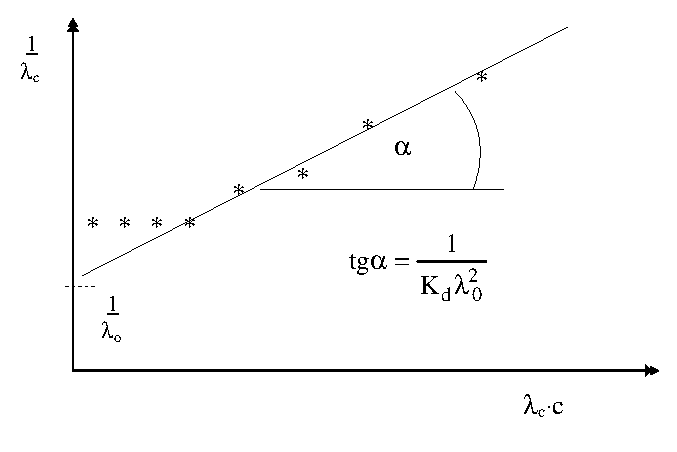
\includegraphics{lambda0.eps}
\caption{Végtelen higítású oldat vezetésének ($\lambda_0$) meghatározása.}
\label{fig:}
\end{figure}

\subsection{A gyakorlat leírása}

A konduktométer harangelektródját többször (4 - 5) öblítsük át desztillált vízzel majd kis részlet 1 $\upmu$S/cm-nél kisebb fajlagos vezetésű vízzel, melyet külön edényben a technikustól kell kérni.
A gyakorlatvezető által kijelölt alkohollal (metanol, etanol vagy propanol) készítsünk 20 v/v\%-os oldatot.
A kijelölt 1 mol$\cdot$dm$^{-3}$ koncentrációjú gyengesav törzsoldatából pipettázzunk két száraz 100 cm$^3$-es mérőlombikba 2.00 cm$^3$-t, majd töltsük jelre az első lombikot vezetőképességi vízzel, a másikat a 20\%-os alkohol oldattal.
A mérést mérőhengerben végezzük.

Töltsük először a vizes hígítású oldatot a mérőedénybe, és mérjük meg a vezetését.
Ezután 25 cm$^3$-t pipettázzunk ki az oldatból és 50 cm$^3$-es mérőlombikban hígítsuk kétszeresére.
Az elektród gondos leöblítése után mérjük ezen oldat vezetését is.
%Az oldat vezetését leghelyesebb úgy meghatározni, hogy az elektród bemerítésétől 5 percen át 30-60 másodpercenként észleljük és feljegyezzük a cellában jelentkező vezetés értékeket.
A kétszeres hígítást még 3-4-szer megismételjük, minden alkalommal mérve a vezetést.

Ismételjük meg a méréseket az alkoholt tartalmazó oldatokkal is úgy, hogy a hígítások során bidesztillált víz helyett a mérőlombikot az alkoholos oldattal töltjük mindig jelre.

Minden esetben jegyezzük fel a mért oldat hőmérsékletét is (a vezetőképességmérő írja az elektródba épített hőmérő által mért hőmérsékletet).
%A mérőcellában egy-egy oldatot legalább 25 percig kell termosztálni.
%A rendelkezésre álló idő rövidsége miatt a legcélszerűbb, ha a sorozat következő, már meghígított tagját főzőpohárban előre a termosztátba helyezzük, így csökkentve a két mérés közti várakozási időt.

Végül mérjük meg mind a hígításokhoz használt vezetőképességi víz, mind az alkohol oldat vezetését, melyekkel mérési eredményeinket korrigálnunk kell.
Ezután határozzuk meg 0.1 és 0.01 M KCl oldatok felhasználásával a cellaállandó értékét úgy, hogy cellakonstansként a két mérésből számolt értékek átlagát fogadjuk el.

A \ref{fig:vez}. ábra egy vezetőképesség mérésére szolgáló cella felépítését mutatja.
A mérendő oldatba egy geometriailag jól definiált, indifferens elektródpárt merítünk és az ezen létrejövő feszültségesést mérjük.
A konduktometria gyakorlatban az elektrolízis, ill. az elektromos polarizáció csökkentése, ill. kiküszöbölése érdekében váltóárammal végezzük a mérést.

\begin{figure}
\centering
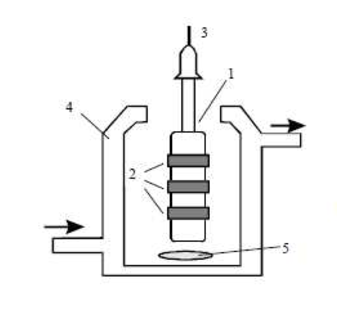
\includegraphics{cond.eps}
\caption{Vezetőképesség mérésére szolgáló cella felépítése. 1 - harangelektród, 2 - Pt korommal bevont gyűrűk, 3 - elektromos elvezetés, 4 - kettős falú temperálható edény, 5 - mágneses keverő.}
\label{fig:vez}
\end{figure}



\subsection{A mérési eredmények kiértékelése}

\begin{enumerate}
\item Számítsuk ki a cellaállandó értékét.
A mérési eredményeket a vizes és az alkoholos sorozatnál is foglaljuk táblázatba:

\begin{table}[!h]
\centering
\begin{tabular}{|c|c|c|c|c|c|c|c|}
\hline
c (mol $\cdot$ dm$^{-3}$) & G$_{\text{mért}}$ & $\kappa_{\text{korr}}$ (S $\cdot$ cm$^{-1}$) & $\lambda_c$ & $1/\lambda_c$ & $\lambda_c c$ & $\alpha$ & $K_d$ \\
\hline
... & ... & ... & ... & ... & ... & ... & ... \\
\end{tabular}
\label{table:vez}
\end{table}

\item Határozzuk meg grafikusan $\lambda_0$ értékét, $\lambda_c$ és $\lambda_0$ ismeretében pedig minden koncentrációra számítsuk ki $\alpha$ és $K_d$ értékeit.

\end{enumerate}



\end{document}
